% ┌                                                ┐
% │     AUTHOR: Janis Hutz<info@janishutz.com>     │
% └                                                ┘

\newsection
\subsection{Fehlerabschätzungen}

\begin{definition}[]{Konvergenz}
    \begin{multicols}{2}
        \fhl{Algebraische Konvergenz}\\
        Wenn der Fehler $E(n) = \tco{\frac{1}{n^p}}$ mit $p > 0$ ist

        \fhl{Exponentielle Konvergenz}\\
        Wenn der Fehler $E(n) = \tco{q^n}$ mit $0 \leq q < 1$
    \end{multicols}
\end{definition}

\numberingOff
\inlineex Zur Fehlerbetrachtung verwenden wir drei Funktionen $f : [0, 1] \rightarrow \R$, welche wir mit trigonometrischer Interpolation an den Punkten $\frac{k}{N}$ approximieren:
\begin{enumerate}[label=(\Roman*)]
    % FIXME: Possibly wrong function definition in script
    \item Stufenfunktion (periodische Fortsetzung von $f$) $f : [0, 1] \rightarrow \R$ mit $f(t) = \begin{cases}
                  0 & \text{für } \left| t - \frac{1}{2} \right| > \frac{1}{4}    \\
                  1 & \text{für } \left| t - \frac{1}{2} \right| \leq \frac{1}{4}
              \end{cases}$
    \item Periodische, glatte Funktion $h: \R \rightarrow \R$ mit $h(t) = \displaystyle \frac{1}{\sqrt{1 + \frac{1}{2} \sin(2\pi t)}}$
          % TODO: Is it $h$ or $g$ here? $g$ makes little sense imho
    \item Hutfunktion (periodische Fortsetzung von $h$) $g : [0, 1] \rightarrow \R$ mit $g(t) = \left| t - \frac{1}{2} \right|$
\end{enumerate}
Die untenstehende Abbildung \ref{fig:interpolation-error-examples} beinhaltet einen Plot, auf dem die Konvergenz in Abhängigkeit des Grades des Interpolationspolynoms aufgetragen ist.
\numberingOn

\begin{figure}[h!]
    \begin{center}
        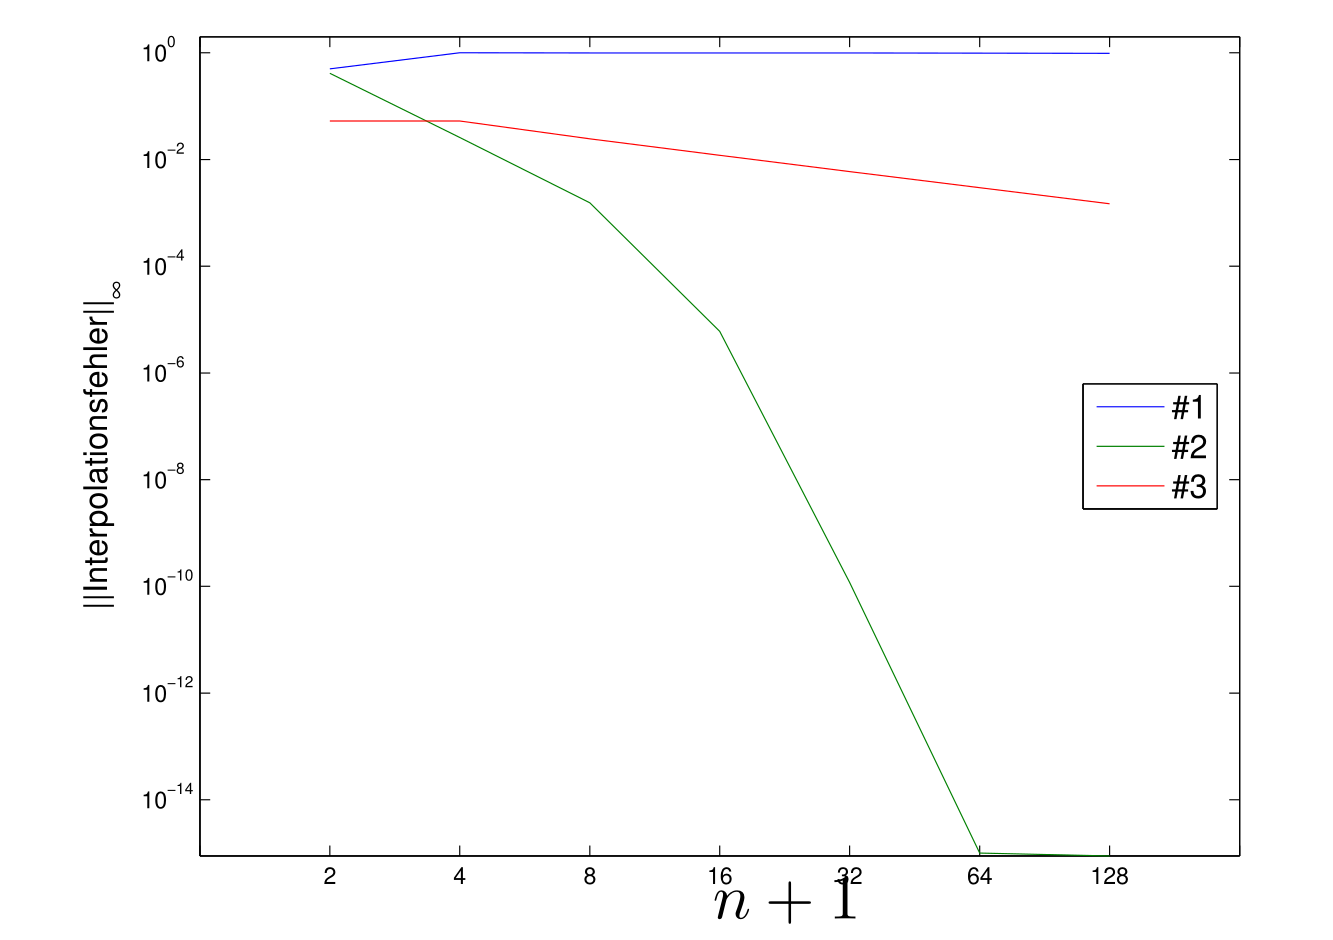
\includegraphics[width=0.6\textwidth]{assets/01_interpolation/01_trigonometric/interpolation-error-examples.png}
    \end{center}
    \caption{Interpolierungsfehler der Beispiele. Algebraische Konvergenz für (I) und (III), exponentielle für (II).
    (Abbildung 3.5.2 aus dem Vorlesungsdokument von Prof. V. Gradinaru, Seite 96)}
    \label{fig:interpolation-error-examples}
\end{figure}
Auch hier tritt das Gibbs-Phänomen wieder an den Sprungstellen von $f(t)$ auf.
Dies verursacht die Verlangsamung der Konvergenz in den Stellen, in welchen die Funktion nicht glatt ist.

\newpage
\stepLabelNumber{all}
\inlineex Sei für $\alpha \in [0, 1)$ $\displaystyle f(t) = \frac{1}{\sqrt{1 - \alpha \sin(2\pi t)}}$.
Die Konvergenz ist exponentiell in $n$ und je kleiner $\alpha$, desto schneller ist sie.
In der untenstehenden Abbildung \ref{fig:interpolation-error-convergence} sind einige Beispiele aufgetragen:
\begin{figure}[h!]
    \begin{center}
        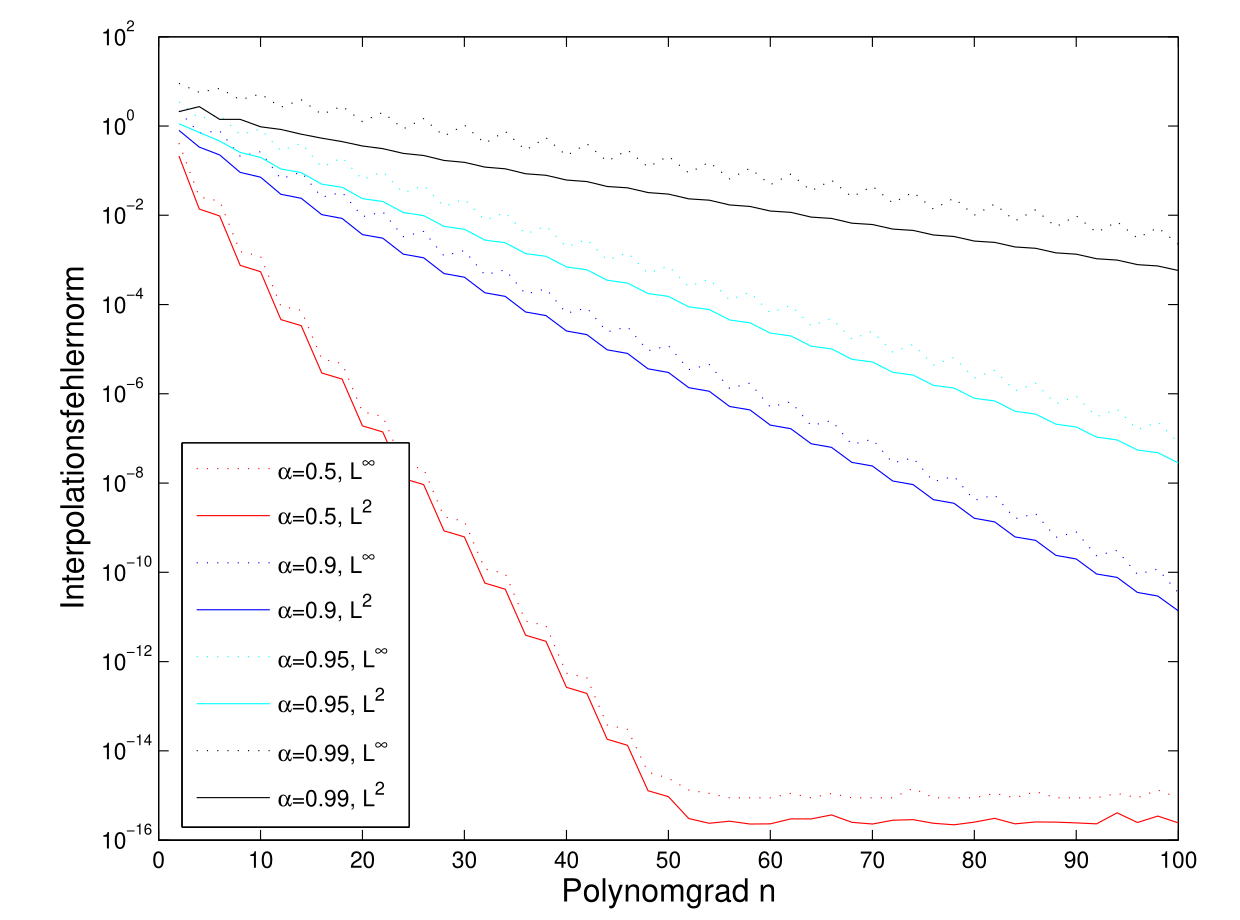
\includegraphics[width=0.6\textwidth]{assets/01_interpolation/01_trigonometric/interpolation-error-convergence.png}
    \end{center}
    \caption{Fehler bei der trigonometrischen Interpolation.
    (Abbildung 3.5.5 aus dem Vorlesungsdokument von Prof. V. Gradinaru, Seite 98)}
    \label{fig:interpolation-error-convergence}
\end{figure}


\setLabelNumber{all}{6}
\begin{theorem}[]{Aliasing}
    Der k-te Fourier-Koeffizient des $N$-ten trigonometrischen Interpolationspolynoms unterscheidet sich vom $k$-ten Fourier-Koeffizienten von $f$ 
    gerade um die Summe aller Fourier-Koeffizienten, die um ganze Vielfache von $N$ vom $k$-ten Fourier-Koeffizienten verschoben sind:
    \begin{align*}
        \hat{p}_N(k) - \hat{f}(k) = \sum_{j \neq 0 \in \Z} \hat{f}(k + jN)
    \end{align*}
\end{theorem}
% FIXME: On page 98, just below the above theorem, there is a text I have no idea what he meant to say... in all honesty, I don't think he was sober when he wrote that

\inlinecorollary Für $f \in \C^p([0, 1])$ mit $p \geq 1$ und $f$ $1$-periodisch, dann gilt: $|\hat{p}_N(k) - \hat{f}(k)| = \tco{(N^{-p})}$ für $|k| \leq \frac{N}{2}$

Das heisst also, dass die Fourier-Koeffizienten von $f$ bei kleinen Frequenzen $\left( \text{hier } |k| < \frac{N}{2} \right)$
sehr gut durch die Fourier-Koeffizienten des trigonometrischen Interpolationspolynoms approximiert werden.

\begin{theorem}[]{Fehler der trigonometrischen Interpolation}
    Falls $f$ $1$-periodisch ist und die Reihe $\sum_{k \in \Z} |\hat{f}(k)|$ absolut konvergiert, dann ist der Approximationsfehler definiert als:
    \begin{align*}
        |p_N(x) - f(x)| \leq 2 \sum_{|k| \geq \frac{N}{2}} |\hat{f}(k)| \mediumhspace \forall x \in \R
    \end{align*}
\end{theorem}
Da durch diesen Satz die obere Schranke für den Approximationsfehler durch die schwer approximierbaren Fourier-Koeffizienten $\hat{f}(k)$ gegeben ist,
heisst das folgendes für die Approximation von Polynomen von Grad $\deg(P(x)) < n$ für unser Approximationspolynom von Grad $\deg(P_N(x)) = n$:

\fancycorollary{Abtasttheorem} Sei $f$ $1$-periodisch mit maximaler Frequenz $m$, also $\hat{f}(k) = 0 \smallhspace \forall |k| > m$. Falls $N > 2m$, dann gilt $p_N(x) = f(x) \smallhspace \forall x$

\numberingOff
\inlineex Ein Beispiel aus der Musik: Wir haben ein analoges Signal und wollen es digitalisieren. 
Wir messen die Spannungswerte in äquidistanten Punkten. 
Falls wir jedoch die Frequenz der Messung zu niedrig wählen, so kann ein total falsches Interpolationspolynom entstehen,
wie in der untenstehenden Abbildung \ref{fig:aliasing} zu sehen:
\numberingOn
\begin{figure}[h!]
    \begin{center}
        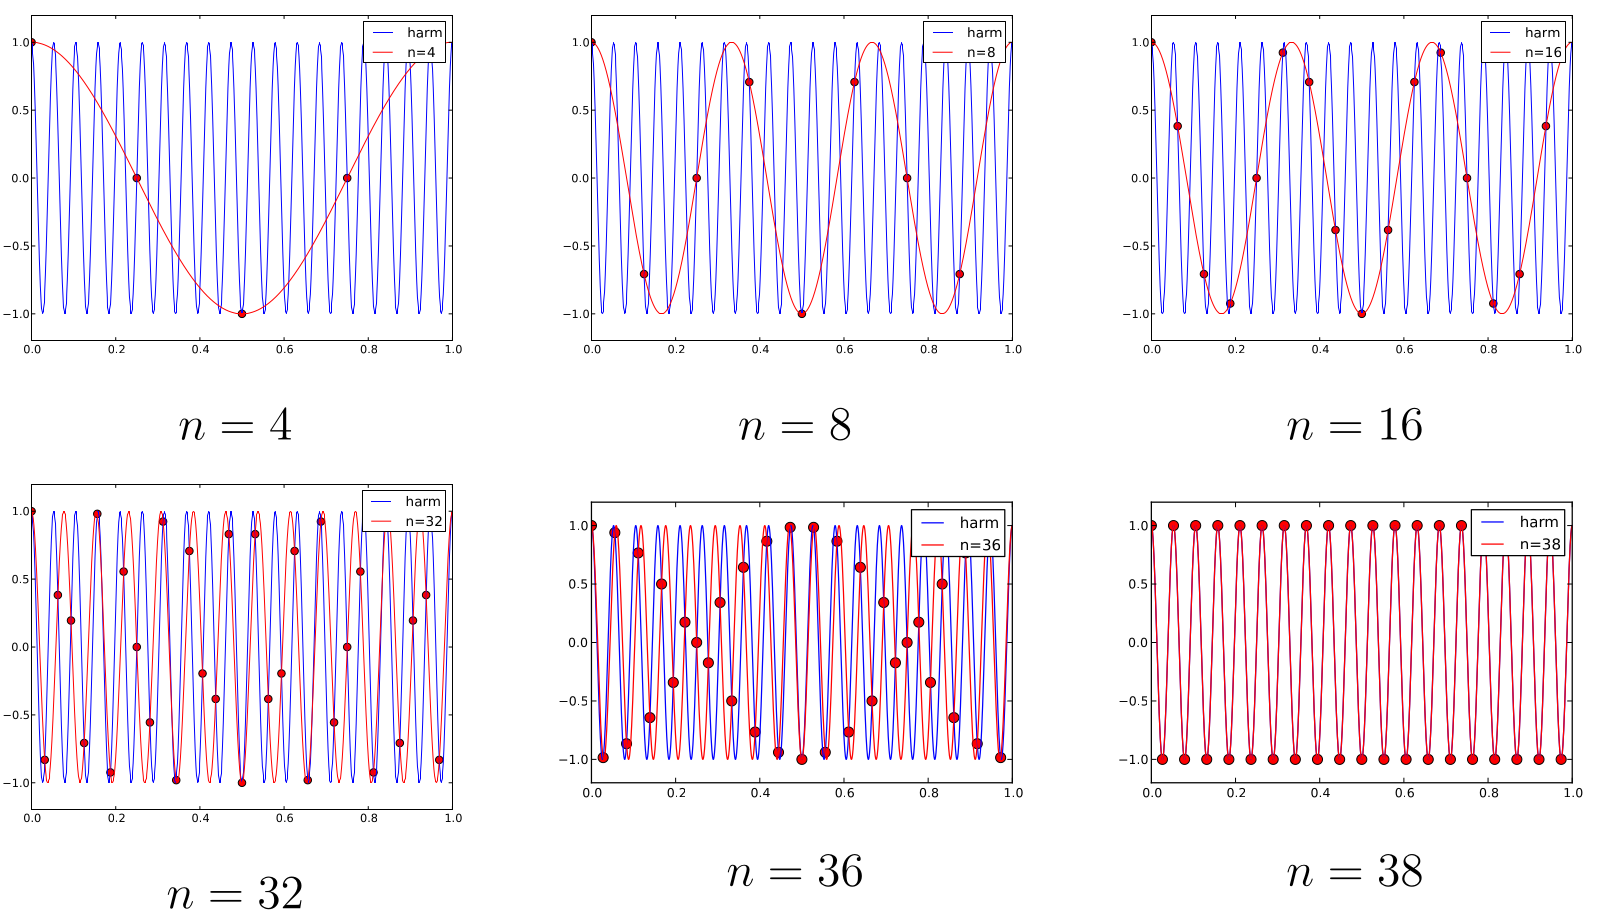
\includegraphics[width=0.95\textwidth]{assets/01_interpolation/01_trigonometric/aliasing-in-music.png}
    \end{center}
    \caption{Aliasing für $f(t) = \cos(2\pi \cdot 19t)$. (Abbildung 3.5.10 aus dem Vorlesungsdokument von Prof. V. Gradinaru, Seite 100)}
    \label{fig:aliasing}
\end{figure}
Für unser Signal bedeutet das also, dass wir eine Art Verzerrung auf der Aufnahme haben, oder für Autoräder, dass es so scheint, als würden sich die Räder rückwärts drehen.

\begin{theorem}[]{Fehlerabschätzung}
    Sei $f^{(k)} \in L^2(0, 1) \smallhspace \forall k \in \N$, dann gilt:
    \rmvspace
    \begin{align*}
        ||f - p_N(f)||_{L^2(0, 1)} \leq \sqrt{1 + c_k} N^{-k} ||f^{(k)}||_{L^2(0, 1)} \text{ wobei } c_k = 2 \sum_{l = 1}^{\infty} (2l - 1)^{-2k}
    \end{align*}
\end{theorem}
Also, je mehr Ableitungen in $L^2(0, 1)$ liegen, desto kleiner ist der Fehler.


Im Skript auf Seiten 101 und 102 gibt es einige Abbildungen die eine gewisse Intuition hinter der Approximation und den entstandenen Fehlern gibt.

